\chapter{Evaluation}

 In this chapter, the author investigates the efficiency of the allocation method proposed in the previous chapter, under the distributed quantum computing system with several processors with different execution time in a limited network topology.  
 
\section{Settings}
In this experiment, three 2-qubit quantum processors with different execution time are connected in a linear topology.
 
 \begin{figure}[ht]
  		\begin{center}
  			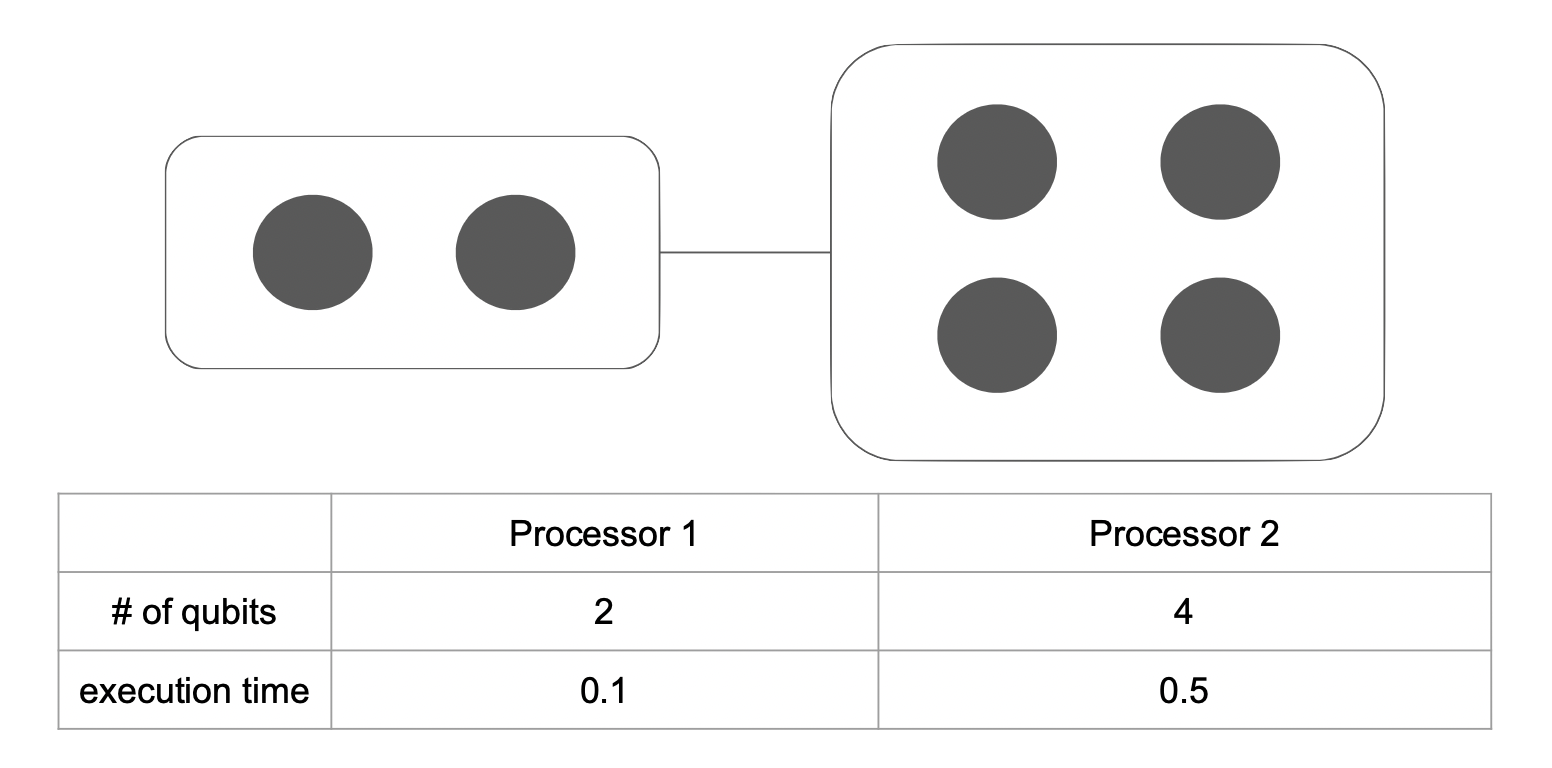
\includegraphics[width=8cm]{img/first_experiment.png}
			\caption{The details of each quantum processor}
		\end{center}
	\end{figure}
 
 The author executed the following circuit on these three quantum processors.  This circuit is a quantum circuit for encoding 5-qubit quantum repetition code, which is one of the circuits used for benchmarking purposes \cite{qasmbench}.
 
  \begin{figure}[ht]
  	\begin{center}
		 \begin{tikzpicture}
  			 \begin{yquant}
      qubit {$\ket{\reg_{\idx}}$} q[5];
      
      h q[0];
      h q[1];
      h q[2];
      h q[3];
      h q[4];
      box {$T$} q[2];
      h q[2];
      h q[2];
      cnot q[2] | q[1];
      cnot q[2] | q[0];
      h q[0];
      h q[1];
      cnot q[2] | q[3];
      h q[2];
      h q[3];
      cnot q[2] | q[3];
      cnot q[2] | q[0];
      cnot q[2] | q[1];
      h q[2];
      cnot q[2] | q[4];
      h q[2];
      h q[4];
      cnot q[2] | q[4];
      cnot q[2] | q[1];
      cnot q[2] | q[3];
      
        			\end{yquant}
		\end{tikzpicture}
	\end{center}
\end{figure}

\newpage
\section{Result}
This experiment was executed using the distributed quantum computing simulator heqsim (Heterogeneous quantum computing simulator) \cite{heqsim}. The author compared the total execution time of three different allocation cases, which are 
 
 \begin{quote}
 \begin{itemize}
  \item when qubits are randomly allocated
  \item when only the gate execution cost is optimized
  \item when only the communication cost is optimized
  \item when both costs are optimized
 \end{itemize}
\end{quote}

I measured the total execution time in the four cases, ten trials for each, and compared the average execution time.  Here is the experiment result.

  \begin{figure}[h]
  		\begin{center}
  			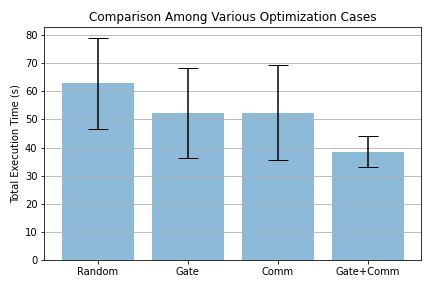
\includegraphics[width=10cm]{img/first_experiment_plot.png}
			\caption{Result}
		\end{center}
\end{figure}

The figure shows that when the both costs are optimized outperforms the three other cases.
 
%%% Local Variables:
%%% mode: japanese-latex
%%% TeX-master: "../bthesis"
%%% End:
